% Use the following line _only_ if you're still using LaTeX 2.09.
%\documentstyle[icml2013,epsf,natbib]{article}
% If you rely on Latex2e packages, like most moden people use this:
\documentclass{article}

% This loads the required math packages.
\usepackage{amsmath}
\usepackage{amsfonts}
\usepackage{amssymb}

% For figures
\usepackage{graphicx} % more modern
%\usepackage{epsfig} % less modern
\usepackage{subfigure} 

% For citations
\usepackage{natbib}

% For algorithms
%\usepackage{algorithms}
\usepackage{algorithmic}

% As of 2011, we use the hyperref package to produce hyperlinks in the
% resulting PDF.  If this breaks your system, please commend out the
% following usepackage line and replace \usepackage{icml2013} with
% \usepackage[nohyperref]{icml2013} above.
\usepackage{hyperref}

% Packages hyperref and algorithmic misbehave sometimes.  We can fix
% this with the following command.
\newcommand{\theHalgorithm}{\arabic{algorithm}}

% Employ the following version of the ``usepackage'' statement for
% submitting the draft version of the paper for review.  This will set
% the note in the first column to ``Under review.  Do not distribute.''
\usepackage{icml2013} 
% Employ this version of the ``usepackage'' statement after the paper has
% been accepted, when creating the final version.  This will set the
% note in the first column to ``Proceedings of the...''
% \usepackage[accepted]{icml2013}


% The \icmltitle you define below is probably too long as a header.
% Therefore, a short form for the running title is supplied here:
\icmltitlerunning{Large-Scale Analysis of Document Similarity Measures of Financial Statements}

\begin{document} 

\twocolumn[
\icmltitle{Large-Scale Analysis of Document Similarity Measures of Financial Statements}

\icmlauthor{Reginald Edwards}{reggie@umich.edu}
\icmladdress{University of Michigan,
            701 Tappan St, Ann Arbor, MI 48109 USA}

% You may provide any keywords that you 
% find helpful for describing your paper; these are used to populate 
% the "keywords" metadata in the PDF but will not be shown in the document
\icmlkeywords{H.3.3 [\textbf{Information Systems}]: Information Search and
Retrieval; I.2.6 [\textbf{Artificial Intelligence}]: Learning; I.2.7
[\textbf{Artificial Intelligence}]: Natural Language Processing—
Text analysis}

\vskip 0.3in
]
%%%%%%%%%%%%%%%%%%%%%%%%%%%%%%%%%%%%
\begin{abstract} 
In this paper I design and implement a system for the retrieval, parsing, and 
clustering based on document similarity of a large web-based corpus of 
documents. Using corporate filings from the United States Securities and 
Exchange Commission EDGAR database, I construct a measure of document 
similarity and implement a fast, scalable, distributed system for the calculation 
of the similarity measure. I validate the empirical usefulness of the textual 
similarity measure in a finance context.
\end{abstract} 

\section{Introduction}\label{intro}
There have been many proposed measures of document similarity but the most commonly used measure is that based on ``cosine similarity.''
While the mathematical construction of cosine similarity for text documents is straightforward, the calculation of the measure on real-world documents is non-trivial. This is especially true when the size of the corpus to be analyzed makes calculation on a single local machine impractical. Therefore, I describe an implementation using a cloud-based distributed platform. Namely, the Elastic Compute Cloud (EC2) from Amazon Web Services (AWS).

\section{Cosine Similarity Measure}\label{cossim}
The construction of textual similarity, $SIM$,  between two sets of accounting policy disclosures involves three components. First, denote  the set of all words occurring in the ``Summary of Significant Accounting Policies'' descriptions in a year is $\Omega_t$. We measure a  scalar, $J_t \equiv \vert\vert \Omega_t \vert\vert$, that is, the number of unique words used in  the descriptions of both firms. For each firm $i$ in year  $t$, an ordered binary vector $W_{it}$ is constructed such that each element $W^{(j)}_{it}$ of  $W_{it}$ is one if and only if word $j$ occurs in the given firm's text in the given  year. Let $N_{it} \equiv W_{it}/\vert\vert W_{it} \vert\vert,$ the normalized vector of word  occurrences for each firm-year. For each year, construct a similar vector $U_t$ of size $J_t$ in  which each element $U^{(j)}_t$ is equal to the sum of the number of occurrences of each word $j$  among both sets of text. From this vector, compute a measure of the aggregate  change in text from year $t-1$ to year $t$ as the change in the number of times the word was used. Denote this aggregate word use change variable as  $D_{t-1,t}$. 

Formally,
\begin{equation}
D_{t-1,t} \equiv \bigg\vert\bigg\vert \sum_{j} (U_{j,t} - U_{j, t-1}) \bigg\vert\bigg\vert.
\end{equation}

The textual similarity of a firm's accounting policy disclosures in a year is constructed as
\begin{equation}
SIM_{it} \equiv \frac{W_{it}}{\vert\vert W_{it} \vert\vert} \cdot \frac{D_{it}}{\vert\vert D_{it} 
\vert\vert},
\end{equation}
which is the cosine of the angle between the firms' vectors of word occurrences and the aggregate word change vector.

In subsequent analysis I make use of a measure of a firm's \emph{self} similarity, 

\begin{equation} SELF \text{-} SIM_{it} \equiv 1 - \frac{W_{it}}{\vert \vert W_{it} \vert \vert} \cdot \frac{W_{it}}{\vert \vert W_{it} \vert \vert}, \end{equation}

which attempt to measure the degree to which the firm is changing its description of its own accounting policies from one year to the next. By construction,  the similarity measure is on the closed interval from zero to one. 

% computation of pairwise cossim
% summary stats: n-gram analyses
\begin{figure}[ht]
\vskip 0.2in
\begin{center}
\centerline{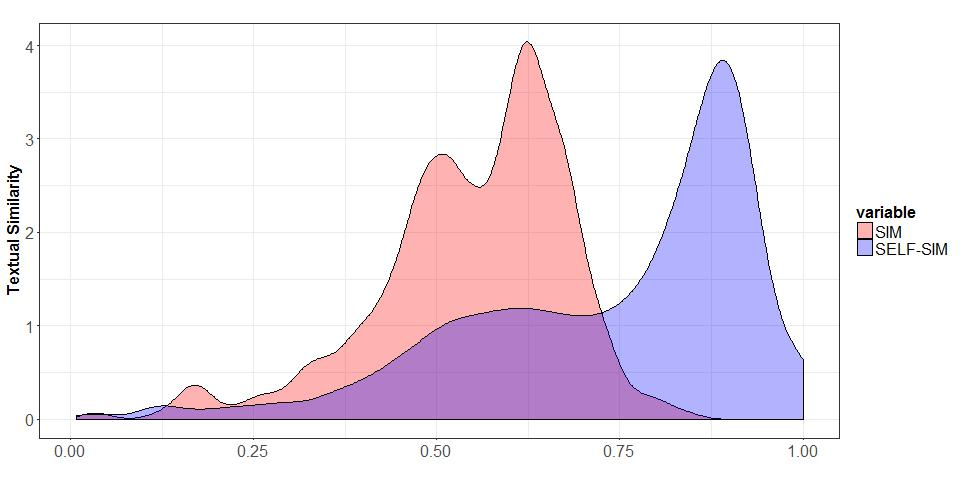
\includegraphics[width=\columnwidth]{figures/cossim-dist}}
\caption{(Top panel) Time series trends of accounting comparability measure $SIM$. (Bottom panel) Pooled cross-sectional distribution of $SIM$.}
\label{cossim-figures}
\end{center}
\vskip -0.2in
\end{figure} 

\section{Implementation}\label{implementation}
\subsection{Data Retrieval from EDGAR}
Number of files
File size distribution (Mb, tokens)
Arrangement of files into years, industry pairs
Distribution of pairs for which cosine similarity will be calculated
\subsection{Cluster Setup}
\subsection{Preprocessing}\label{ssec:preprocess}
% steps to download 10-K's. Discuss attrition, compustat matching
% steps to extract SAP, discuss attrition. Summary stats to show representativeness (ts, xs, industry)
% lemmatization and stemming
To more accurately analyze the 10-K sections I perform several preprocessing steps on the corpus. Specifically, I remove alphanumeric sequences and punctuation, convert all words to lowercase, and perform stemming and lemmatization on each document.
Stemming and lemmatization are methods from the fields of computational linguistics and natural language processing that are designed to normalize textual corpora for automated analyses. Stemming requires to conversion of a word token to its root, removing pluralization and conjugation. Lemmatization is designed to convert word tokens that are different but often used to refer to the same physical entity to a common token. 

Below is an example from the 2011 annual report of IBM. The filing originally contained the line:

\begin{quote}
Additionally, changes to noncontrolling interests in the Consolidated Statement of Changes in Equity were \$(29) million, \$8 million and \$(1) million for the years ended December 31, 2011, 2010 and 2009, respectively
The accounts of variable interest entities (VIEs) are included in the Consolidated Financial Statements, if required.
\end{quote}

After the pre-processing steps described above, the line became:

\begin{quote}
addit chang noncontrol interest consolid statement chang equiti million million million year end decemb respect account variabl interest entiti vie includ consolid financi statement requir
\end{quote}

To reduce further the amount of irrelevant information contained in each piece of text extracted from the 10-K, I weight each word token that occurs via a method known as term frequency-inverse document frequency (tf-idf). This weighting scheme reduces the influence of overly common terms in a text corpus on the analysis of that corpus. These steps should reduce the amount of noise in the construction of accounting similarity.

\subsection{Calculation of Cosine Similarity}

\section{Datasets and Validation}\label{data}
Publicly traded firms in the United States are required to file detailed annual reports, which are subsequently made available to the public. These annual reports, known as ``10-K's'' from the Securities and Exchange Commission form number of the report, must contain descriptions of the operations of the firm, financial results, and the accounting treatment used to prepare the financial statements. By accounting treatment, it is meant the set of allowed accounting rules chosen by the firm to recognize revenues and expenses and to measure assets and liabilities. Firms discuss these accounting treatments in the section of the 10-K known as the ``Summary of Significant Accounting Policies,''  which itself is a subsection of the ``Notes to the Financial Statements'' (henceforth ``the notes''). The accounting policies section is typically the first subsection of the notes, which themselves typically are the first section after the financial statements (balance sheet, income statements, statement of cash flows, and statement of shareholders' equity). 

\begin{table}[t]													
 \caption{Univariate Determinants of Accounting Comparability. This table presents univariate regression results of $SIM$ on firm characteristics. $SIM_{t-1}$ indicates the one-year lag of similarity. All other variables are as defined in Appendix A.}
 \label{cossim-uni}																				
\vskip 0.15in
\begin{center}
\begin{small}
\begin{sc}
\begin{tabular}{lrrrr}
  \hline
\abovespace\belowspace
 & Coeff & Std Err & \emph{t} & $R^2$\\ 
  \hline
\abovespace
AGE & 0.00 & 0.00 & 2.05 & 0.02 \\ 
AT & 0.00 & 0.00 & 6.08& 0.16 \\ 
BASPREAD & -0.33 & 0.05& -6.37 & 0.17 \\ 
MVE & 0.00 & 0.00 & 6.38 & 0.17 \\ 
PE & -0.00 & 0.0 & -2.40 & 0.02 \\ 
SP500 & -0.01 & 0.00 & -5.51 & 0.13 \\ 
TANG & -0.01 & 0.01 & -1.85 & 0.01 \\ 
TURNOVER & 0.00 & 0.0 & 10.48 & 0.46 \\ 
$SIM_{t-1}$ & 0.65 & 0.01 & 111.73 & 38.33 \\
   \hline
\end{tabular}
\end{sc}
\end{small}
\end{center}
\vskip -0.1in
\end{table}

In this paper I find novel evidence that the accounting policies section contains significant predictive content in an financial context. Namely, I find that the similarity of these texts is predictive of the behavior of large institutional investors. Institutional investors are large investors who often trade on behalf of a large number of individuals. Such institutions make up the vast majority of dollars invested in public equity markets.

\section{Results}\label{results}
\section{Related Work}\label{lit}
\section{Conclusions}\label{conclusions}

% Acknowledgements should only appear in the accepted version. 
\section*{Acknowledgments} 
 
This work is based, in part, on my doctoral dissertation at the University of Michigan Ross School of Business. I would like to thank my dissertation committee chairs Raffi Indjejikian and Venky Nagar and members Allison Earl and Robert F. Dittmar. I am also grateful for the advice and comments of Ryan Ball, Greg Miller, Cathy Shakespeare, Christopher Williams, and Reuven Lehavy, as well as workshop participants at the University of Michigan. I appreciate the financial support of the Ross Doctoral Fellowship, the Paton Accounting Fellowship, and the University of Michigan Rackham Merit Fellowship.

\bibliography{example_paper}
\bibliographystyle{icml2013}

\end{document}